\chapter{Executive Summary }
\label{ch:project-overview}
\section{Overview}
The Deep Underground Neutrino Experiment (DUNE) will be a world-class neutrino observatory and nucleon decay detector designed
to answer fundamental questions about the nature of elementary particles and their role in the universe. 
The DUNE far detector will be located about one mile underground at the Sanford Underground Research 
Facility (SURF) in South Dakota, at a distance of \SI{1300}{\km} from Fermilab, and
will be a very large, modular liquid argon time-projection chamber (LArTPC) with a fiducial mass of 40 ktons. 
This liquid argon technology will make it possible to reconstruct neutrino interactions with image-like precision
and unprecedented resolution.

The far detector will be exposed to
the world's most intense neutrino beam originating at Fermilab. 
A high-precision near detector, located 575~m from the neutrino source on the Fermilab site, will be used to characterize the intensity and energy spectrum of this wide-band beam
The Long Baseline Neutrino Facility (LBNF) provides the infrastructure for this complex system of detectors at the Fermilab and SURF sites.
LBNF combines the responsibility for the neutrino beam, 
the deep-underground site, and the infrastructure for the DUNE detectors.

%%%%%%%%%%%%%%%%%%%%%%%%%%%%%%%%%%%%%%%%%%%%%%%%%%%%%%%%%%%%%%%
%\section{International Context}

\begin{dunefigure}[DUNE Collaboration Global Map]{fig:mhexec}{The international DUNE
Collaboration}
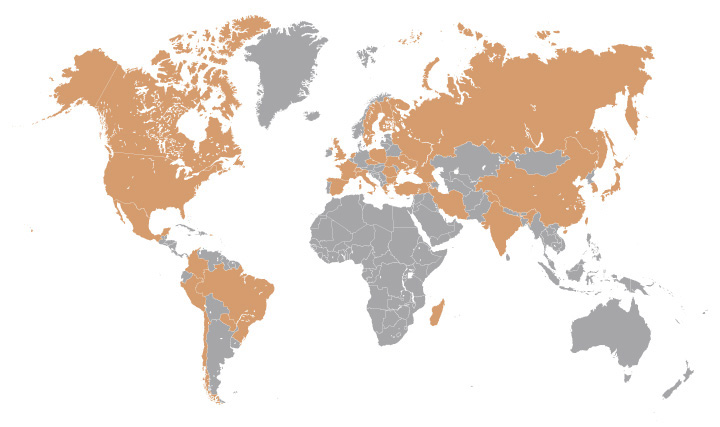
\includegraphics[width=0.9\textwidth]{global.jpg}
\label{fig:map}
\end{dunefigure}

The DUNE Collaboration is a truly global organization including more than 1000 scientists and engineers from 31 countries (Figure~\ref{fig:map}). It represents
the culmination of several worldwide efforts that developed independent paths toward a next-generation long-baseline neutrino experiment over the last decade.
It was formed in April 2015, combining the strengths of the LBNE project in the US and the LBNO project in Europe, adding many new international 
partners in the process. DUNE thus represents the convergence of a substantial fraction of the worldwide neutrino-physics community around the 
opportunity provided by the large investment planned by the U.S. Department of Energy (DOE) to support 
a significant expansion of the underground infrastructure at the Sanford Underground Research 
Facility (SURF) in South Dakota, and to create a megawatt neutrino-beam facility at Fermilab by 2026. 
The PIP-II upgrade~\cite{pip2-2013}
will enable the accelerator to drive the new neutrino beamline with a beam power\footnote{assuming a \SI{120}{\GeV} primary proton beam. 
For a \SI{80}{\GeV} primary proton beam, the corresponding beam power is \SI{1.07}{\MW}.} of up to \SI{1.2}{\MW}. A further planned upgrade 
of the accelerator complex will enable it to provide up to \SI{2.4}{\MW} of beam power by 2030.  

The LBNF/DUNE project (the ``project'') strategy presented in this technical proposal has been developed to meet the requirements set out in the report of the Particle Physics Project Prioritization Panel (P5). It also takes into account the recommendations of the European Strategy for Particle  Physics (ESPP) adopted by CERN Council in 2013, which classified the long-baseline neutrino program as one of the four scientific objectives that required international infrastructure.
%which recommends development of
%a program to pave the way for a substantial European role in future long-%baseline experiments.

The P5 report set the goal of reaching a sensitivity to CP violation of better than 3$\sigma$ over more than $75\%$ 
of the range of possible values of the unknown CP-violating phase \deltacp.
Based partly on this goal, they stated that ``the 
minimum requirements to proceed are the identified capability to reach an exposure 
of \num{120}~\ktMWyr{} by the 2035 time frame, the far detector situated underground 
with cavern space for expansion to at least 40~kt LAr fiducial volume, and 1.2~MW 
beam power upgradeable to multi-megawatt power.
The experiment should have the demonstrated 
capability to search for supernova bursts and for proton decay, providing a significant 
improvement in discovery sensitivity over current searches for the proton lifetime.'' The strategy and design presented in this technical proposal meets these requirements.
%Based on the resource-loaded schedules for the reference designs of the facility %(\vollbnf)
%and the detectors, %(\voldune), 
%the strategy presented here meets these criteria. 

%The physics case for LBNF and DUNE was highlighted as a strategic priority in the 2014 report
%by the Particle Physics Project Prioritization Panel (P5), which defines the long-term strategy and priorities for U.S. investments 
%in particle physics~\cite{p5report2014}. These recommendation are in line with the 
%European Strategy for Particle Physics (ESPP) adopted in 2013~\cite{ESPP-2012} which recommends to develop 
%a program to pave the way for a substantial European role in future long-baseline experiments.

%The P5 report identifies the  minimum requirements for LBNF to proceed: 
%the identified capability to reach an exposure of at least 120~\ktMWyr{}~\footnote{An exposure
%of 1 MW.year corresponds to $1\times 10^{21}$ protons-on-target per year at 120 GeV. This includes the LBNF beamline efficiency which is estimated to be 56\%.}  by the 2035 timeframe;
%the far detector situated underground with cavern space for expansion to at least 40-kt LAr fiducial;
%1.2-MW beam power upgradeable to multi-megawatt power;
%demonstrated capability to search for supernova bursts; and
%a demonstrated capability to search for proton decay, 
%providing a significant improvement in discovery sensitivity over current searches for the proton lifetime.
%Furthermore, P5 identified the goal of a sensitivity to CP violation of better than 3$\sigma$ over more than $75\%$ 
%of the range of possible values of the unknown CP-violating phase \deltacp.

%The strategy and design choices presented in this TP meet all of these requirements.

This document presents 
a Technical Proposal (TP) developed by an international collaboration of scientists and engineers to construct DUNE,
a groundbreaking science experiment for long-baseline neutrino oscillation studies, neutrino astrophysics, and nucleon decay searches. As will be described in the final section of this executive summary, this technical proposal for the DUNE far detectors is an intermediate milestone toward the production of a full technical design report (TDR) about one year later.


%

%%%%%%%%%%%%%%%%%%%%%%%%%%%%%%%%%%%%%%%%%%%%%%%%%%%%%%%%%%%%%%%%
\section{Primary Science Goals (Ed)}


The DUNE experiment will combine the world's most intense neutrino beam, a deep underground site, and massive LAr detectors to enable a broad science program addressing some of the most fundamental questions in particle physics. 

%Searches for CP violation in neutrino oscillations may give insight into the origin of the matter-antimatter asymmetry, one of the fundamental questions in particle physics and cosmology. Detection of neutrinos from a nearby supernova could provide a wealth of information about neutrinos and the dynamics of supernovae. Observation of proton decay would dramatically change our understanding of particle physics

The primary science goals of DUNE, described in detail in Chapter~\ref{ch:exec-summ-physics}, are to
\begin{itemize}

\item Carry out a comprehensive program of neutrino oscillation measurements using $\nu_mu$ and ${\overline \nu_mu}$ beams from Fermilab. This program includes measurements of the CP phase, determination of the neutrino mass ordering (the sign of $\Delta m^2_{31} \equiv m_3^2-m_1^2$), measurement of the mixing angle $\theta_{23}$ and the determination of the octant in which this angle lies,
and sensitive tests of the 3-neutrino paradigm. Paramount among these is the search for CP violation in neutrino oscillations, which may give insight into the origin of the matter-antimatter asymmetry, one of the fundamental questions in particle physics and cosmology. 

\item Search for proton decay in several important decay modes, such as $\text{p}\rightarrow\text{K}^+\overline{\nu}$. The observation of proton decay would represent a ground-breaking discovery in physics, providing a key requirement for Grand Unification of the forces. 

    \item Detect and measure the $\nu_\text{e}$ flux from a core-collapse supernova within our galaxy, should one occur during the lifetime of the DUNE experiment. Such a measurement would provide a wealth of unique information about the early stages of core-collapse, and could even signal the birth of a black hole.
    
\end{itemize}

The intense neutrino beam from LBNF, the massive DUNE LArTPC far detector, and the high-resolution
DUNE near detector will also provide a rich ancillary science program, beyond the primary goals of the experiment. The ancillary science program includes
\begin{itemize}
     \item other accelerator-based neutrino flavor transition measurements with sensitivity to Beyond Standard Model (BSM) physics, such as non-standard interactions (NSIs), CPT violation, sterile neutrinos, large extra dimensions, heavy neutral leptons;
 and measurements of tau neutrino appearance;
     \item measurements of neutrino oscillation phenomena using atmospheric neutrinos;
     \item a rich neutrino interaction physics program utilizing the DUNE near detector, including a wide-range of measurements of neutrino cross sections, studies of nuclear effects, including neutrino final-state interactions, measurements of the structure of nucleons, and  measurement of $\sin^2\theta_\text{W}$;
     \item  searches for dark matter.
\end{itemize} 
Further developments of LArTPC %far detector 
technology during the course of the DUNE far detector construction may open up the opportunity
to observe very low-energy phenomena such as solar neutrinos or even the diffuse supernova neutrino flux.

%Searches for CP violation in neutrino oscillations may give insight into the origin of the matter-antimatter asymmetry, one of the fundamental questions in particle physics and cosmology. Detection of neutrinos from a nearby supernova could provide a wealth of information about neutrinos and the dynamics of supernovae. Observation of proton decay would dramatically change our understanding of particle physics.


%The phenomenon of neutrino oscillations stands as one of the most important recent discoveries in particle physics, and the realization that neutrinos are massive particles remains the only discovery of phenomena beyond the original formulation of the Standard Model.  
%Neutrinos are the second most abundant particle in the universe, yet one of the most difficult to detect.  What they have told us already, about themselves and the rest of the Standard Model, has revolutionized particle physics.  
%Neutrino experiments are now poised to address some of the most fundamental questions in science.  Paramount among these is the search for CP violation in the neutrino sector, which may give insight into the origin of the matter-antimatter asymmetry. The Deep Underground Neutrino Experiment (DUNE) will make comprehensive measurements of neutrino and anti-neutrino oscillations to test CP invariance in the lepton sector, determine the ordering of the neutrino mass eigenstates, and perform precision tests of the neutrino Standard Model.  DUNE will take advantage of both an accelerator-based neutrino beam from Fermilab and be sensitive to extra-terrestrial neutrinos, including from supernova explosions.  DUNE's massive, underground detector, a 40-kton Liquid Argon Time Projection Chamber (LAr-TPC), will both enable these precision measurements in neutrino physics and astrophysics as well as extend the sensitivity in the search for nucleon decay. 

%The study of the properties of neutrinos has produced
%many surprises, including evidence for physics beyond the Standard Model of elementary particles and interactions. The phenomenon of neutrino flavor oscillations, whereby 
%neutrinos can transform into a different flavor after traveling a distance, %change flavor as they propagate through space and time, 
%is now well established. Important conclusions that follow from these discoveries include that neutrinos have mass and that their %the 
%mass eigenstates are mixtures of their %the 
%flavor eigenstates.

%Speculations on the origin of neutrino masses and mixings are wide-ranging. 
%Solving the puzzle will require more precise and detailed experimental information with neutrinos and antineutrinos, and with sensitivity to matter effects. With the exception of a few anomalous results, the current data can be described in terms of the three-neutrino paradigm, in which the 
%quantum-mechanical mixing of the three mass eigenstates produces the three known neutrino-flavor states.  The mixings are described by the Pontecorvo-Maki-Nakagawa-Sakata (PMNS) matrix, a parameterization that includes a CP-violating phase. 

%The primary science objectives %goals 
%of DUNE are to carry out a comprehensive investigation of neutrino oscillations to test CP violation in the lepton sector, determine the ordering of the neutrino masses, and to test the three-neutrino paradigm.
%By measuring \textit{independently} the  propagation of neutrinos and antineutrinos through matter, DUNE will be able to observe %measure the 
%neutrino transitions with the precision required to determine the 
%CP-violating phase and %determine 
%the neutrino mass hierarchy.

% moved up At the same time, t
%The construction of LBNF and DUNE will also enable a high-priority ancillary science program, including
%very precise measurements of neutrino interactions and cross-sections, studies of nuclear effects in such interactions, measurements of the structure of nucleons, as well as precise tests of the electroweak theory. 
%These measurements of the properties of neutrino interactions are also necessary 
%\fixme{will allow DUNE (per SP)} %are essential 
%to achieve the best sensitivities in the long-baseline neutrino oscillation program. %studies. \
%At the same time, the massive DUNE far detector,located deep underground, 
%each with a mass forty times %an order of magnitude 
%larger than ever built,  
%  MAT: note ICARUS T600 consisted of two 300 t modules each with a fiducial mass of ~440 t
%    ---  %realized, 
%will offer unique capabilities for addressing 
%non-accelerator physics topics. These include measuring atmospheric neutrinos, searching for nucleon decay, and measuring astrophysical neutrinos --- possibly even %especially 
%the neutrino burst %those 
%from a core-collapse supernova. 
%produced by such supernovae and atmospheric neutrinos will be detected and measured in ways that 
%Observations of these kinds will bring new insight into these fascinating natural phenomena. 



%An intriguing %attractive 
%conjecture is that of neutrino masses being related to an %new 
%ultra-high-energy scale that may be associated with the unification of matter and forces. Such theories are able to describe the absence of antimatter in the universe in terms of the properties of ultra-heavy particles; they also % as well as offering 
%offer an explanation %a description 
%of cosmological inflation in terms of the phase transitions associated with the breaking of symmetries at this ultra-high-energy scale. DUNE's capability to detect and study rare events such as nucleon decays in an unbiased and unprecedented way will allow it to probe these very high-energy scales. 



%Finally, further developments of LArTPC %far detector 
%technology during the course of the DUNE far detector construction may open up the opportunity
%to observe very low-energy phenomena such as solar neutrinos or even the diffuse supernova neutrino flux.



%%%%%%%%%%%%%%%%%%%%%%%%%%%%%%%%%%%%%%%%%%%%%%%%%%%%%%%%%%%%%%%
\section{The LBNF Facility} %Global LBNF/DUNE Strategy}

The Long-baseline Neutrino
Facility (LBNF) is separate from the DUNE Collaboration and is intended to enable the construction and operation of the DUNE detector.
The DUNE Collaboration will construct a deep-underground neutrino observatory based on four independent \ktadj{10} LArTPCs at the Sanford Underground Research Facility (SURF) in South Dakota.
LBNF will provide facilities at Fermilab and at SURF to enable the scientific program of DUNE.
These facilities are geographically separated into the Near Site Facilities, those to be constructed
at Fermilab, and the Far Site Facilities, located at SURF. Figure~\ref{fig:lbnf} shows
a schematic of the facilities at Fermilab and SURF. 

\begin{dunefigure}[ 	
LBNF/DUNE project: beam from Fermilab to the Sanford Underground Research Facility]{fig:lbnf}{ 	
LBNF/DUNE project: beam from Fermilab to the Sanford Underground Research Facility}
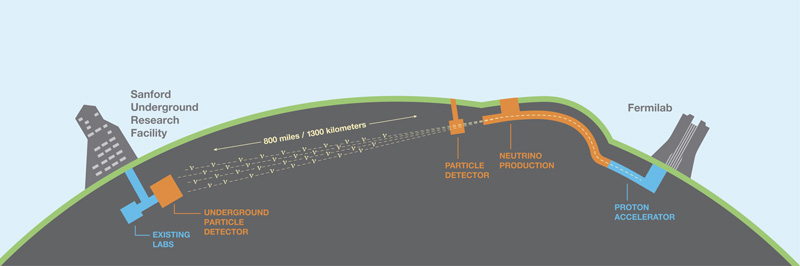
\includegraphics[width=0.9\textwidth]{lbnf_dune_graphic_miles_km-15-0031-01.jpg}
%\label{fig:mhexec}
\end{dunefigure}

Specifically, the Long-Baseline Neutrino Facility (LBNF) provides
\begin{itemize}

\item  the  technical and conventional facilities for a powerful \MWadj{1.2} neutrino beam utilizing the PIP-II upgrade of the Fermilab accelerator 
complex, to become operational by 2025 
at the latest, and to be upgradable to \SI{2.4}{\MW} with the proposed 
PIP-III upgrade;

\item  the civil construction (conventional facilities or CF) for the near detector systems at Fermilab; 

\item the excavation of four underground caverns at SURF, planned to be completed 
by 2021 
under a single contract, with each cavern to be capable of housing a cryostat for
a minimum \ktadj{10} fiducial mass LArTPC; and
%\fixme{changed per SP}


\item surface, shaft, and underground infrastructure to support 
the outfitting of the caverns with four free-standing, steel-supported cryostats 
and the required cryogenics systems. The first cryostat will be available for filling, after installation of the detector components, by
2023, enabling a rapid deployment of the first two \ktadj{10} far detector modules. 
The intention is to install the third and fourth cryostats as rapidly as funding will 
allow.

\end{itemize}
The success of the DUNE project will depend on the successful realization of the LBNF facilities.
This Technical Proposal focuses on the DUNE physics program that is enabled by
the first three Far Detector modules, which are expected to be based on the single-phase and dual-phase liquid-argon technologies. 

\section{The DUNE Experiment (Ed)}

% ecb: Do ProtoDUNEs show up here or in a separate section? Somewhere, we need to state what specific performance measures we are counting on having from ProtoDUNE before the TDR.

The DUNE experiment includes a precision near detector at the edge of the Fermilab site, and a very large, modular far detector about one mile underground at the Sanford Underground Research Facility (SURF) in Lead, South Dakota, 800 miles (1300 km) from Fermilab. The DUNE far detector is the focus of this technical proposal. 

The near detector will be located 575 m from the target. It will consist of a LAr TPC followed by a fine-grained magnetic spectrometer. The LAr TPC will use pixel readout to deal with the high occupancy from neutrino events in the intense LBNF beam. The details of magnetic spectrometer should be resolved in the near future. The goal for the near detector is to produce a conceptual design report (CDR) at the time of the far detector technical design report (TDR). The near detector CDR will provide information critical to establishing the physics reach for the primary neutrino oscillation program of DUNE. The near detector TDR will follow the far detector TDR by about one year, consistent with the near detector construction schedule.

The DUNE far detector will consist of 4 similar liquid argon TPCs, each with fiducial mass of at least 10 ktons, installed about 1 mile underground at SURF. Each detector will be installed in a cryostat with internal dimensions
$15.1 m (W) \times 14.0 m (H) \times 62 m (L)$, and will contain a total mass of about 17 ktons of liquid argon.
The LAr TPC technology provides
excellent tracking and calorimetry performance, making it an ideal
choice for the DUNE far detectors. The four identically sized cryostats give flexibility for staging and evolution of LAr TPC technology.
%for massive neutrino detectors, which require high signal efficiency and effective background discrimination, excellent capability to identify and  precisely measure neutrino events over a wide range of energies, and excellent reconstruction of the kinematical properties of events
%with high resolution. The full imaging of events will allow study of neutrino interactions and other rare events with an unprecedented resolution.
% The huge mass will allow collection of sufficient statistics for precision
%studies, as discussed in Chapter~\ref{v1ch:science}.

DUNE is planning for and prototyping two LAr-TPC technologies:
\begin{itemize}
\item Single-Phase. This technology was pioneered in the context of the ICARUS project, and after several decades of worldwide R\&D, is now a mature technology. It is the technology used for MicroBooNE, and planned for SBND. Ionization charges are drifted horizontally in liquid argon and read out on wires in the liquid. The maximum drift length in the DUNE far detector is 3.6 m and the nominal drift field is 500 V/cm, corresponding to a total HV of 180 kV. There is no signal amplification in the liquid, so readout with good signal-to-noise requires very low-noise electronics.

\item Dual-Phase. The dual-phase technology was pioneered at large scale by the WA105 collaboration. It is less established than than the single phase technology, but offers a number of potential advantages and challenges. Here, ionization charges are drifted vertically in liquid argon and then transfered into the gas above the liquid. The signal charges are then amplified in the gas phase using large electron multipliers (LEMS). This gain reduces the requirements on the electronics, and makes it possible for the dual phase detector to have a longer drift, which requires a correspondingly higher voltage.
The maximum drift length in the DUNE far detector is 12 m and the nominal drift field is 500 V/cm, corresponding to a total HV of 600 kV. 

\end{itemize}
The plans for the single and dual-phase TPCs are described in detail in volumes 2 and 3 of this technical proposal.

The DUNE Collaboration is committed to deploying both technologies. 
For planning purposes, we are assuming that the first far detector module will be
single-phase and the second will be dual-phase.
The actual sequence of detector installation will depend on results from the prototype detectors, described below, and on available resources.


The Collaboration is in now in the final stages of constructing two large prototype detectors (called ProtoDUNEs), one employing single-phase readout and the other employing dual-phase readout. Each ProtoDUNE is approximately 1/20 of a full DUNE module, but uses components identical in size to those of the full-scale module. The single-phase prototype has the same 3.6 m maximum drift length as the full DUNE module. The dual-phase prototype has a 6 m maximum drift length, half of that planned for the DUNE far detector. 

These large-scale prototypes, which are described in more detail in the single-phase and dual-phase volumes of this technical proposal, will allow us to validate key aspects of the TPC designs, test engineering procedures, and collect valuable calibration data using a hadron test beam. The following list includes the key goals of the protoDUNE program:
\begin{enumerate}
\item Test production of components
\begin{itemize}
\item stress testing of the production and quality
assurance processes of detector components
\item mitigate the associated risks for the far detector.
\end{itemize}
\item Validate installation procedures:
\begin{itemize}
\item test of the interfaces between the detector
elements
\item mitigate the associated risks for the far detector.
\end{itemize}
\item Detector Operation with cosmic rays
\begin{itemize}
\item validation of the detector designs and
performance
\end{itemize}
\item Collection of test beam data:
\begin{itemize}
\item essential measurements of physics response of
detector
\item not necessary to finalize the far detector design
\end{itemize}
\end{enumerate}

Items 1 - 3 are required as input to the technical design report. Item 4, collection and the corresponding analysis of test beam data, will be critical to DUNE's physics program, but is not required for the TDR.

As noted above, the full DUNE far detector requires 4 modules. For the TDR, we will describe plans for at least the first two of these modules. Based on our current expectations, we hope to present a plan for 2 single-phase far detector modules, one of which will be the first module installed, and 1 dual-phase far detector module. At the time of the TDR, it is likely that resources for the 4th detector module will remain to be identified. 


%The Deep Underground Neutrino Experiment (DUNE) provides
%\begin{itemize}

%\item four massive LArTPCs, each with a fiducial mass of at least \SI{10}{\kt}. The division of 
%the far detector into four equal-mass detectors provides the project flexibility 
%in the installation and funding (DOE vs. non-DOE); this division also mitigates risks and allows for an early and graded science return.

%\item the near detector systems, consisting of a high-resolution neutrino detector 
%and the muon monitoring system that will enable %necessary to reach 
%the precision %requirements 
%needed to fully 
%exploit the statistical power of the %very massive 
%far detector coupled to the %powerful 
%MW-class 
%neutrino beam.
%\end{itemize}


%Based on the reference design described below and in Volumes 2, 3 and 4 of this %the LBNF/DUNE 
%CDR, the resource-loaded schedule %will see 
%plans for the first two \ktadj{10} far detector modules to be
%operational by 2025,
%with first beam shortly afterward. 
%\fixme{above sentence changed slightly per SP}
%At that time, the cavern 
%space for all four \ktadj{10} far detector modules will be available, %allowing for 
%an accelerated installation schedule if sufficient funding sources for
%the experiment can be established on an accelerated timescale.  

%\vspace{6pt}
%The project strategy described above meets the experiment's scientific objectives,
% reaching an exposure of 
%\num{120}~\ktMWyr{} by 2032, and potentially earlier if additional resources are identified. 
%The P5 recommendation of sensitivity to CP violation of 3$\sigma$ for 75\% of $\delta_\text{CP}$
%values can be reached with an exposure of \num{850}~\ktMWyr{} with an optimized beam.

%%%%%%%%%%%%%%%%%%%%%%%%%%%%%%%%%%%%%%%%%%%%%%%%%%%%%%%%%%%%%%%
\section{International Organization and Responsibilities}

DUNE is the first science project of this scale in the US that will be built with large
international participation. This requires a new organizational and governance model that takes into account the international nature of the project.
The
model used by CERN for managing the construction and exploitation of the Large Hadron Collider (LHC) and its experiments was used as a starting point for the joint management of LBNF and the DUNE experimental program. 
LBNF, which is responsible for the facilities, comprising the neutrino beam, the near site at Fermilab and the far site at SURF, is organized as a
DOE/Fermilab project incorporating international partners. 

DUNE is a fully international project
organized by the DUNE Collaboration with appropriate oversight from all international stakeholders.
The DUNE collaboration is responsible for
\begin{itemize}
\item the definition of the scientific goals and corresponding scientific and technical requirements on the detector systems and neutrino beamline;
\item the design, construction, commissioning and operation of the detectors; and
\item the scientific research program conducted with the DUNE detectors. 
\end{itemize}

A set  of  structures  has been established  to  provide
coordination  among  the  participating  funding agencies;
oversight of the LBNF and DUNE projects;
and coordination and communication between the 
two. These structures and the relationships among them are shown 
in Figure~\ref{fig:org}. The comprise the following committees:
\begin{itemize}
\item International Neutrino Council (INC)

The International Neutrino Council (INC) is composed of regional representatives, such as CERN, and representatives of funding agencies making major contributions to LBNF infrastructure or to DUNE. The INC acts as the highest-level international advisory body to the U.S. Department of Energy (DOE) and the Fermilab Directorate. The INC facilitates high-level global coordination across the entire enterprise (LBNF and DUNE). The INC is chaired by the DOE Office of Science Associate Director for High Energy Physics and includes the Fermilab Director in its membership. The council meets and provides pertinent advice to the LBNF and DUNE projects through the Fermilab Director as needed.
\item Resources Review Board (RRB)

The Resources Review Board (RRB) is composed of representatives of all funding agencies that sponsor LBNF and DUNE, and the Fermilab management. The RRB provides focused monitoring and detailed oversight of each of the projects. The Fermilab Director in coordination with the DUNE Resource Coordinator (RC) defines its membership. A representative from the Fermilab Directorate chairs the RRB and organizes regular meetings to ensure the required flow of resources for the smooth progress and successful completion of the LBNF and DUNE projects. The management teams from the DUNE collaboration and the LBNF project participate in the RRB meetings and make regular reports to the RRB on technical, managerial, financial and administrative matters, as well as reporting on the status and progress of the DUNE Collaboration.

\item Long-Baseline Neutrino Committee (LBNC)

The Long Baseline Neutrino Committee (LBNC) is composed of internationally prominent scientists with relevant expertise. It provides regular external scientific peer review for the two projects. The LBNC reviews the scientific, technical and managerial decisions and preparations of the neutrino program. It acts effectively as an adjunct to the Fermilab PAC, meeting on a more frequent basis than the PAC. The LBNC may employ additional DUNE and LBNF scrutiny groups for more detailed reports and evaluations. 

\item Experiment-Facility Interface Group (EFIG)

Close and continuous coordination between DUNE and LBNF is required to ensure the success of the combined enterprise. The Experiment-Facility Interface Group (EFIG)  oversees and ensures the required coordination both during the design and construction and the operational phases of the program. This group covers areas including interfaces between the near and far detectors and the corresponding conventional facilities; interfaces between the detector systems provided by DUNE and the technical infrastructure provided by LBNF; design of the LBNF neutrino beamline and neutrino beamline operational issues that impact both LBNF and DUNE.  

\end{itemize}





\section{DUNE Organization and Management (Ed)}

All aspects of DUNE are organized and managed by the DUNE collaboration.  Stakeholders include the collaborating institutions, the funding agencies participating in DUNE, and Fermilab as the host laboratory.  All collaborating institutions have a representative on the DUNE Institutional Board (IB). The collaboration is responsible for the design, construction, installation, commissioning, and operation of the detectors and prototypes used to pursue the scientific program. The DUNE Executive Board, described below, is the main management body of the collaboration and approves all significant strategic and technical decisions.

The top-level DUNE Management Team consists of two elected Co-Spokespersons, the Technical Coordinator (TC), and the Resource Coordinator (RC). The TC and RC are selected jointly by the Co-Spokespersons and the Fermilab Director. The Management Team is responsible for the day-to-day management of the collaboration, and for developing the overall collaboration strategy, which is presented for approval to the Executive Board. The Executive Board is made up of the leaders of the main collaboration activities. The composition of the EB, currently including the DUNE management team, the IB chair, the physics coordinator, beam interface coordinator, physics coordinator, computing coordinator, near detector coordinator, and leaders of the far detector consortia, described below, is intended to ensure
that all stakeholders in the collaboration have a voice in the decision-making process. 
In the post-TDR phase of DUNE, the intention is that the Consortium Leaders and the coordinators of the other major collaborations will become elected positions.
%, giving the full collaboration as a whole is represented in the decision-making process. 

To carry out design and construction work for the DUNE far detectors, we formed consortia of institutions that have taken responsibility for different detector subsystems. A similar structure will be formed for the DUNE Near Detector once the detector concept is selected. For the DUNE far detector, there are currently 9 consortia, including 3 specific to single-phase (SP), 3 specific to dual-phase (DP), and 3 common to both technologies:
\begin{itemize}
\item (SP) Anode Plane Assemblies% (C. Touramanis, UK)
\item (SP) TPC Electronics% (D. Christian, US)
\item (SP) Photon Detection System% (E. Segreto, Brazil)
\item (DP) Charge Readout Planes% (D. Duchesneau, France)
\item (DP) TPC Electronics %(D. Autiero, France)
\item (DP) Photon Detection System %(I. Gil-Botella, Spain)
\item HV System %(F. Pietropaolo, CERN)
\item DAQ System %(D. Newbold, UK)
\item Slow Controls and Instrumentation. %(S. Gollapinni, US)
\end{itemize}
It is possible that one or two additional consortia may be added depending on the organization of computing and calibration systems. Each consortium has an overall leader, a technical lead, and a consortium board with representatives from each consortium institution. In addition to a variety of other tasks, the consortia are responsible for writing their respective sections of the technical proposal and the TDR.


%%%%%%%%%%%%%%%%%%%%%%%%%%%%%%%%%%%%%%%%%%%%%%%%%%%%%%%%%%%%%%%
\section{Schedule and Milestones (Stefan)} %Brisk Schedule} %vigorous schedule}
%\fixme{please suggest a better word than vigorous??..Andr\'e}

The schedule for the design and construction work for LBNF and DUNE has two critical parallel paths: one for the %Far Site scope at SURF 
far site (SURF) and %one 
another for the %Near Site scope at 
near site (Fermilab). The schedule for the initial work is driven by the CF design and construction at each site. A summary of the schedule is shown in Figure~\ref{fig:summary-sched}.
%\fixme{SP suggests a figure -- famous Napolean Russian campaign diagram style!}

\begin{dunefigure}[High-level summary of LBNF/DUNE schedule]{summary-sched}{High-level summary of LBNF/DUNE schedule}
%\includegraphics[width=1.2\textwidth, angle=90]{summary-schedule.png}
\end{dunefigure}


Within the anticipated DOE funding profile, in particular during the initial phase of the project, the far site conventional
facilities are advanced first; their final design starts in fall 2015. Early site preparation is timed to be completed 
in time to start excavation when the Ross Shaft rehabilitation work finishes
 in late 2017. As each detector 
 cavern is excavated and sufficient utilities are installed, the cryostat and cryogenics system work proceeds, followed by detector installation, filling and commissioning. 
 The far detector module \#1 is to be operational by 2024 with modules \#2 and \#3 completed
 one and two years later, respectively, and module \#4 completed by early 2027.

The near site work is delayed with respect to the far site due to the anticipated funding profile. The near site CF and beamline work essentially slows to nearly a stop %almost no effort 
until design restarts in late 2017. Optimization decisions about the beamline that affect the CF design will need to be made by late 2018 in order to be ready for the CF design process. The embankment is constructed and then allowed to settle for at least twelve months before the majority of the beamline CF work proceeds. The beneficial occupancies of the various beamline facilities %CF 
are staggered to allow beamline installation to begin as soon as possible. With this timescale, the far detector science program % with the Far Detectors 
starts with the first module installed and no beam, focusing on non-accelerator-based science %, since 
for slightly more than one year until 
the beamline installation is completed.


The near detector CF construction overlaps that for the beamline, but lags due to available funding. The near detector assembly begins on the surface before beneficial occupancy, after which the detector is installed, complete at about the same time as far detector module \#4. 

The DOE project management process requires approvals at Critical Decision milestones, which allow the LBNF/DUNE project to move to the next step. In fall 2015 the far site CF will seek CD-3a approval for construction of some of the CF and cryogenics systems at SURF. In spring 2018 LBNF near site CF will seek CD-3b construction approval for Advanced Site Preparation to build the embankment. In 2020 LBNF and DUNE will seek to baseline the LBNF/DUNE scope of work, cost and schedule, as well as construction approval for the balance of the project scope of work. 

The project concludes with CD-4 approval to start operations.

%%%%%%%%%%%%%%%%%%%%%%%%%%%%%%%%%%%%%%%%%%%%%%%%%%%%%%%%%%%%%%
\section{The DUNE Technical Proposal Volumes}

%%%%%%%%%%%%%%%%%%%%%%%%%%%%%%%%%%%
%\subsection{A Roadmap of the TP}

The DUNE Technical Proposal (TP) describes the proposed physics program and 
technical designs of the facility and detectors in preparation for the full Technical Design Report (TDR)
to be published in 2019.  This TP represents our best knowledge of the final design of the first three far detector modules at this moment
in time. The fourth liquid-argon module could employ a different technology, taking into account lessons learnt from the design of the first modules, to further optimize the sensitivity for physics discoveries. It is beyond the scope of this proposal. This proposal does also not cover the Near Detector, which represents an integral part of DUNE physics programme. A separate TDR for these detectors components will be
provided in the future.

Two prototype liquid-argon detectors, ProtoDUNE Single-phase (SP) and Dual-phase (DP) are currently under construction at CERN.
The experience gained from building and then operating ProtoDUNE using cosmic rays and a charged-particle beam will be crucial for refining and optimizing the design choices to be presented in the TDR. At the same time as writing this TP, the Collaboration
has made fast progress in constructing and assembling the ProtoDUNE detectors, which
are on track to take data later this year. 

The TP is intended as an intermediate
milestone on the path to a full TDR, justifying the technical choices that will enable the DUNE experiment
to make discoveries and answer the flagship physics questions. These technical design choices therefore flow from
the requirements defined by the high-level physics goals.

In addition to this Executive Summary, the TP comprises two volumes describing the two liquid-argon detector 
technologies, as well as the installation and integration plans for the detector.
\begin{itemize}
 \item Single-phase DUNE Far Detector (Volume~2)
 \item Dual-phase DUNE Far Detector (Volume~3)
\end{itemize}
The Executive Summary describes the general aims of this document, In addition, it contains discussions of a possible calibration strategy for the liquid-argon detectors, and of a computing and software model for DUNE. It will then introduce
the primary and ancillary science programs. Volumes 2 and 3 are devoted to the two complementary technology choices for the
liquid-argon detectors. 
